\section{Langkah-Langkah Percobaan}

\begin{enumerate}
    \item Kabel LAN dihubungkan dari laptop ke router, dan router ke router.
    \item Login menggunakan MAC address, lalu router direset terlebih dahulu menggunakan Winbox.
    \begin{figure}[H]
        \centering
        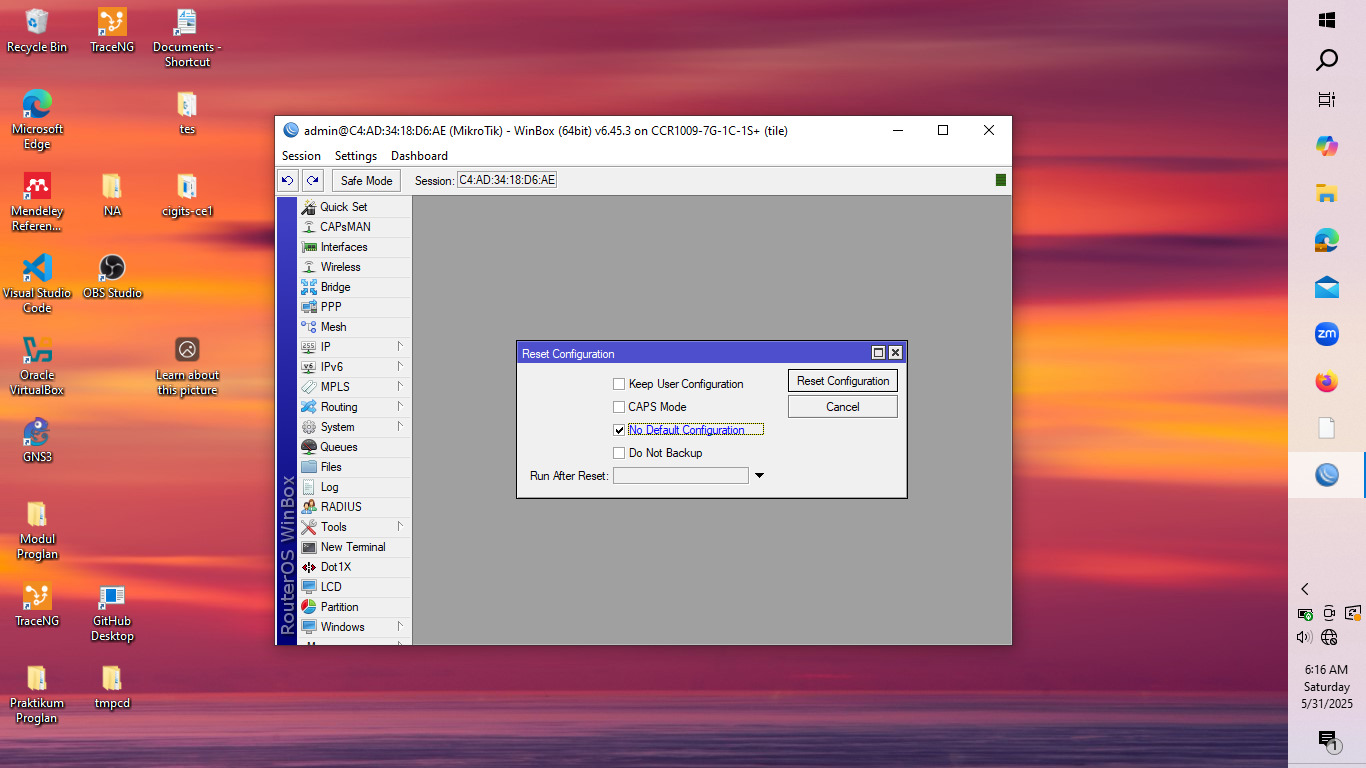
\includegraphics[width=0.5\linewidth]{gambar1.jpeg}
        \caption{Mereset Router pada Winbox}
        \label{fig:reset-router}
    \end{figure}

    \item DHCP dikonfigurasikan 
    \begin{figure}[H]
        \centering
        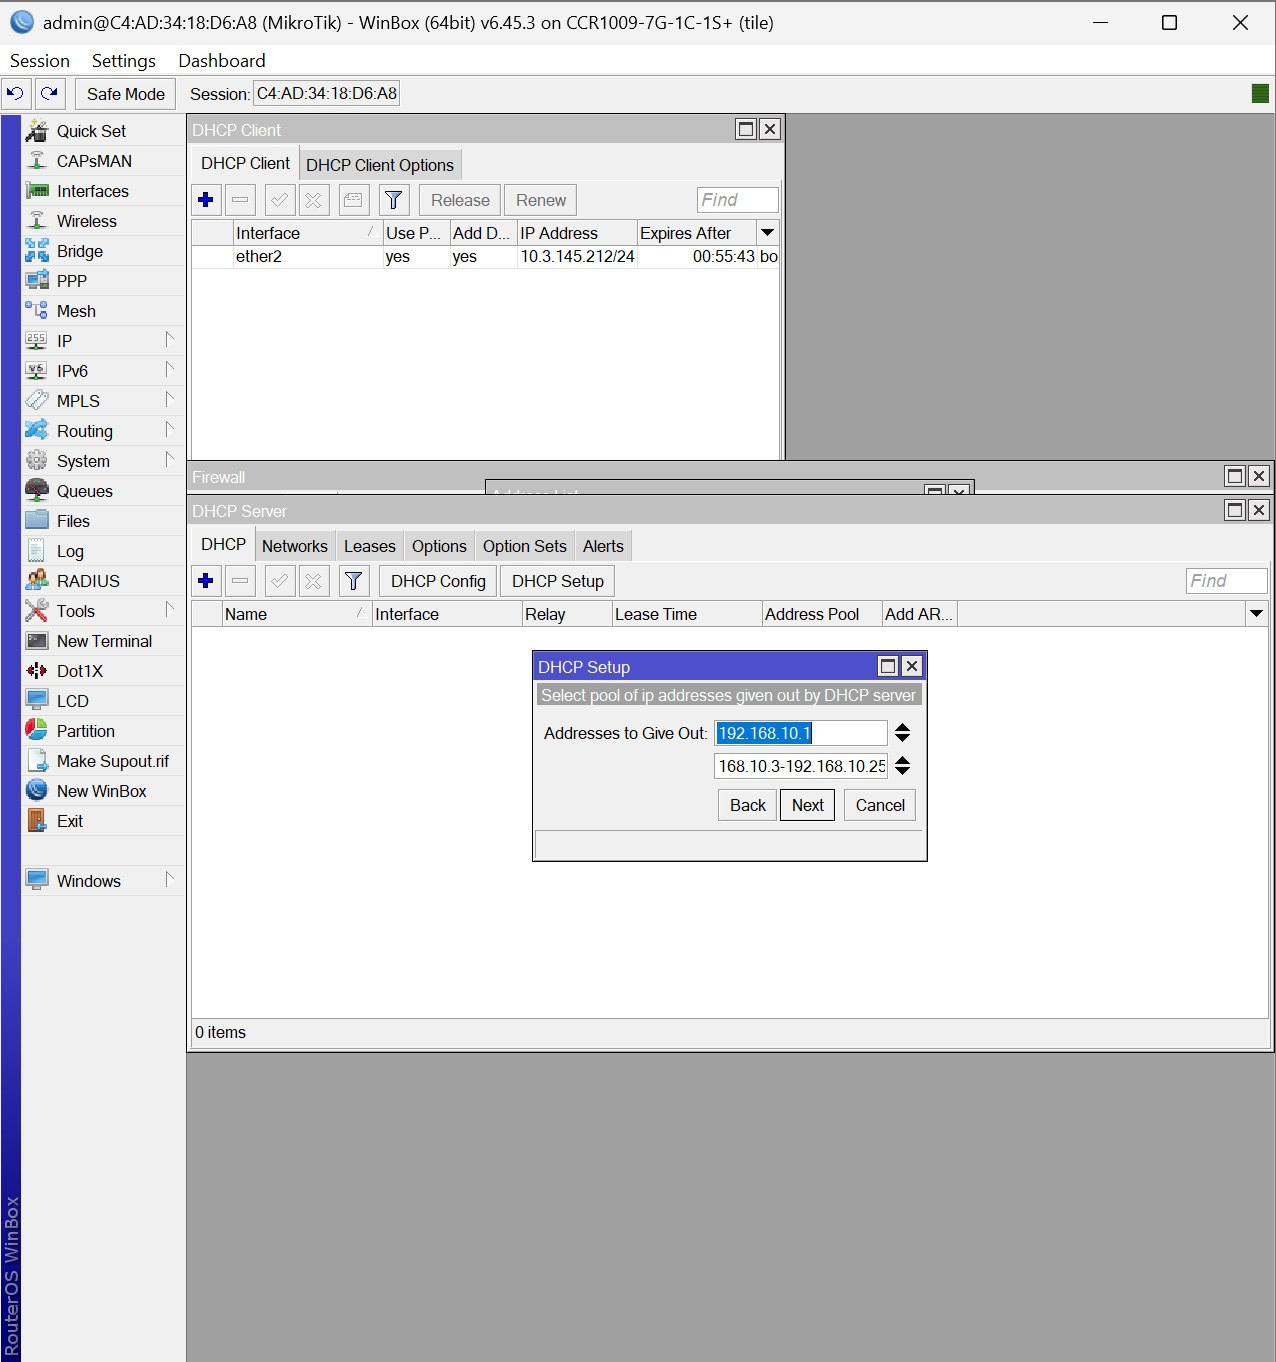
\includegraphics[width=0.5\linewidth]{gambar2.jpeg}
        \caption{Mengkonfigurasi DHCP Client pada Router yang terhubung ke internet}
        \label{fig:DHCP-router-A}
    \end{figure}
    \item Firewall NAT dikonfigurasikan
    \begin{figure}[H]
        \centering
        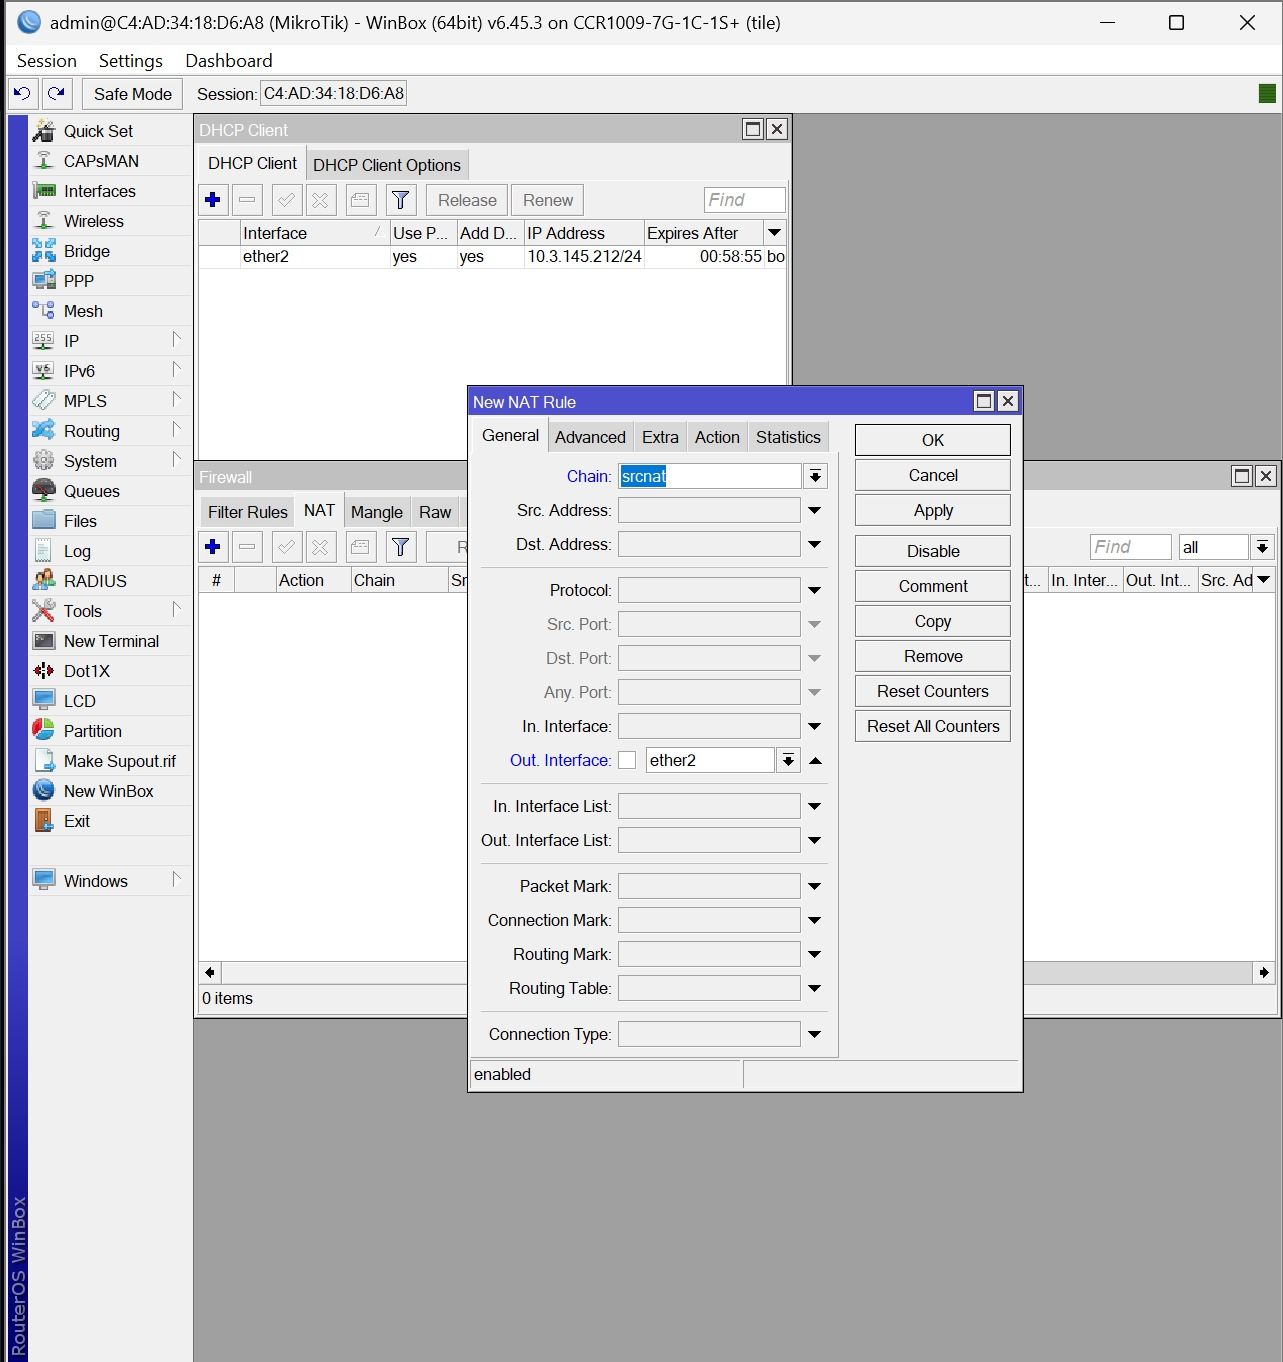
\includegraphics[width=0.5\linewidth]{gambar3.jpeg}
        \caption{Menambahkan Alamat IP pada ether 3}
        \label{fig:Firewall-NAT}
    \end{figure}
    \item Alamat IP dikonfigurasikan untuk jaringna lokakl yang akan terhubung ke ether 1
    \begin{figure}[H]
        \centering
        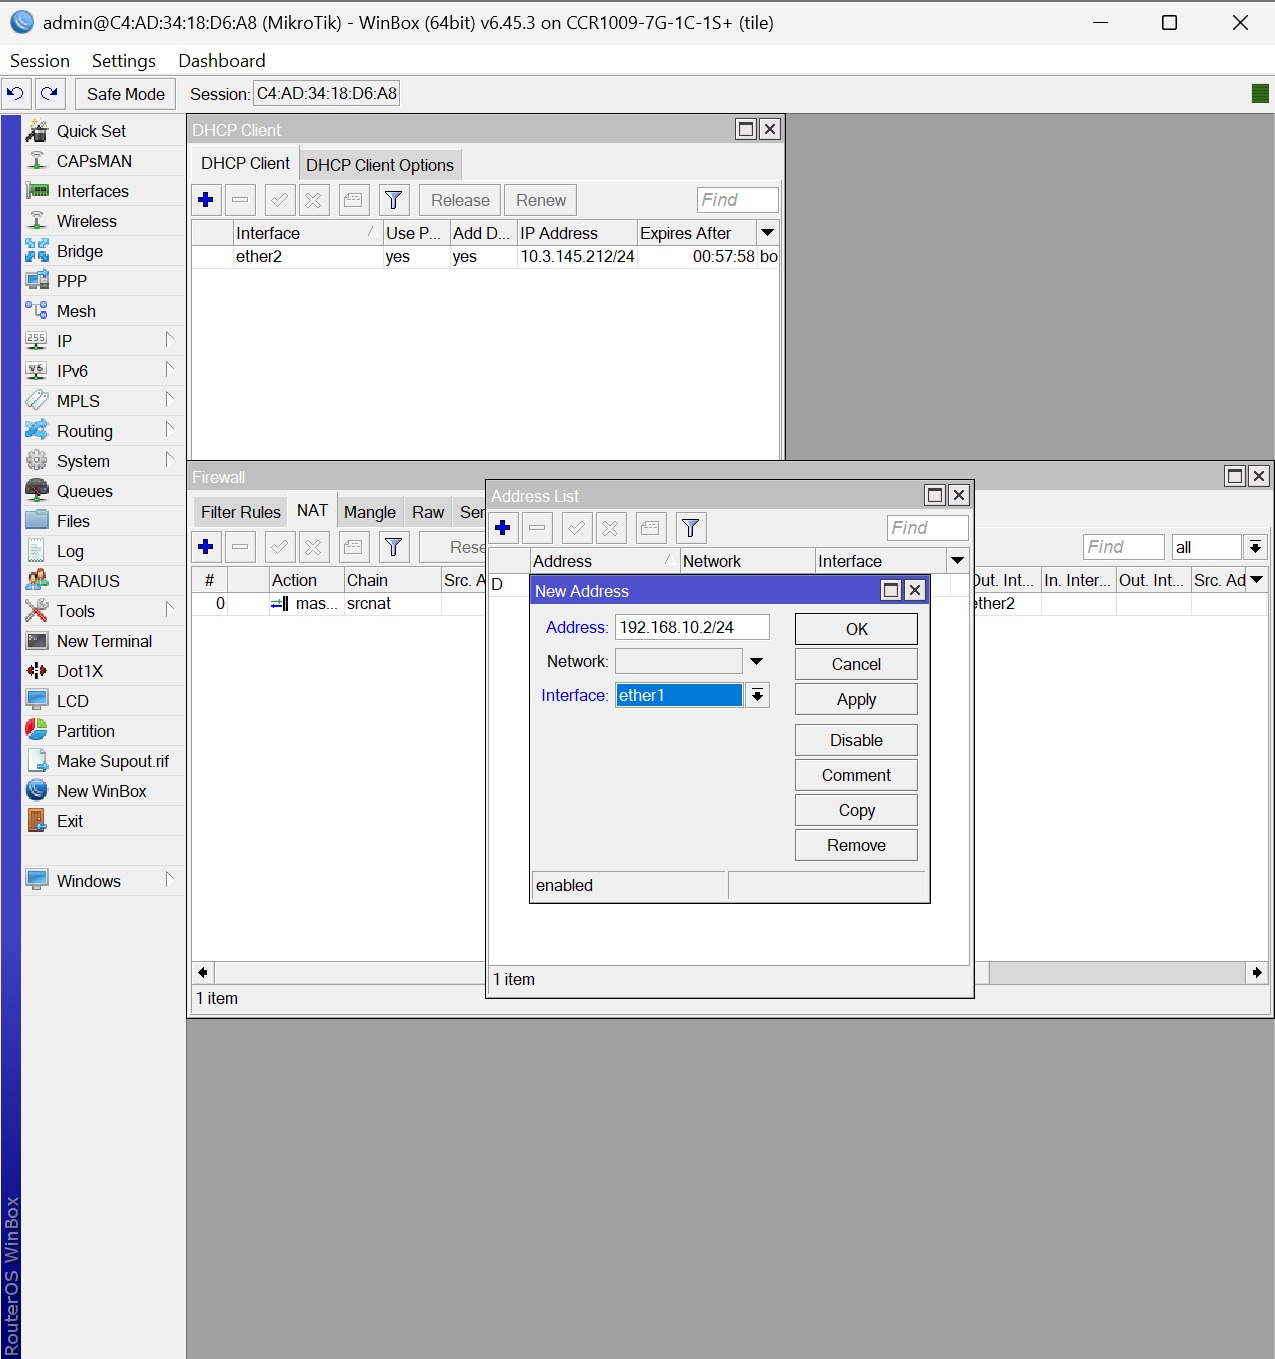
\includegraphics[width=0.5\linewidth]{gambar4.jpeg}
        \caption{Mengkonfigurasikan DHCP server pada mikrotik}
        \label{fig:Alamat-IP-ether}
    \end{figure}
    \item Konfigurasi DHCP server untuk distribusi IP klien 
    \begin{figure}[H]
        \centering
        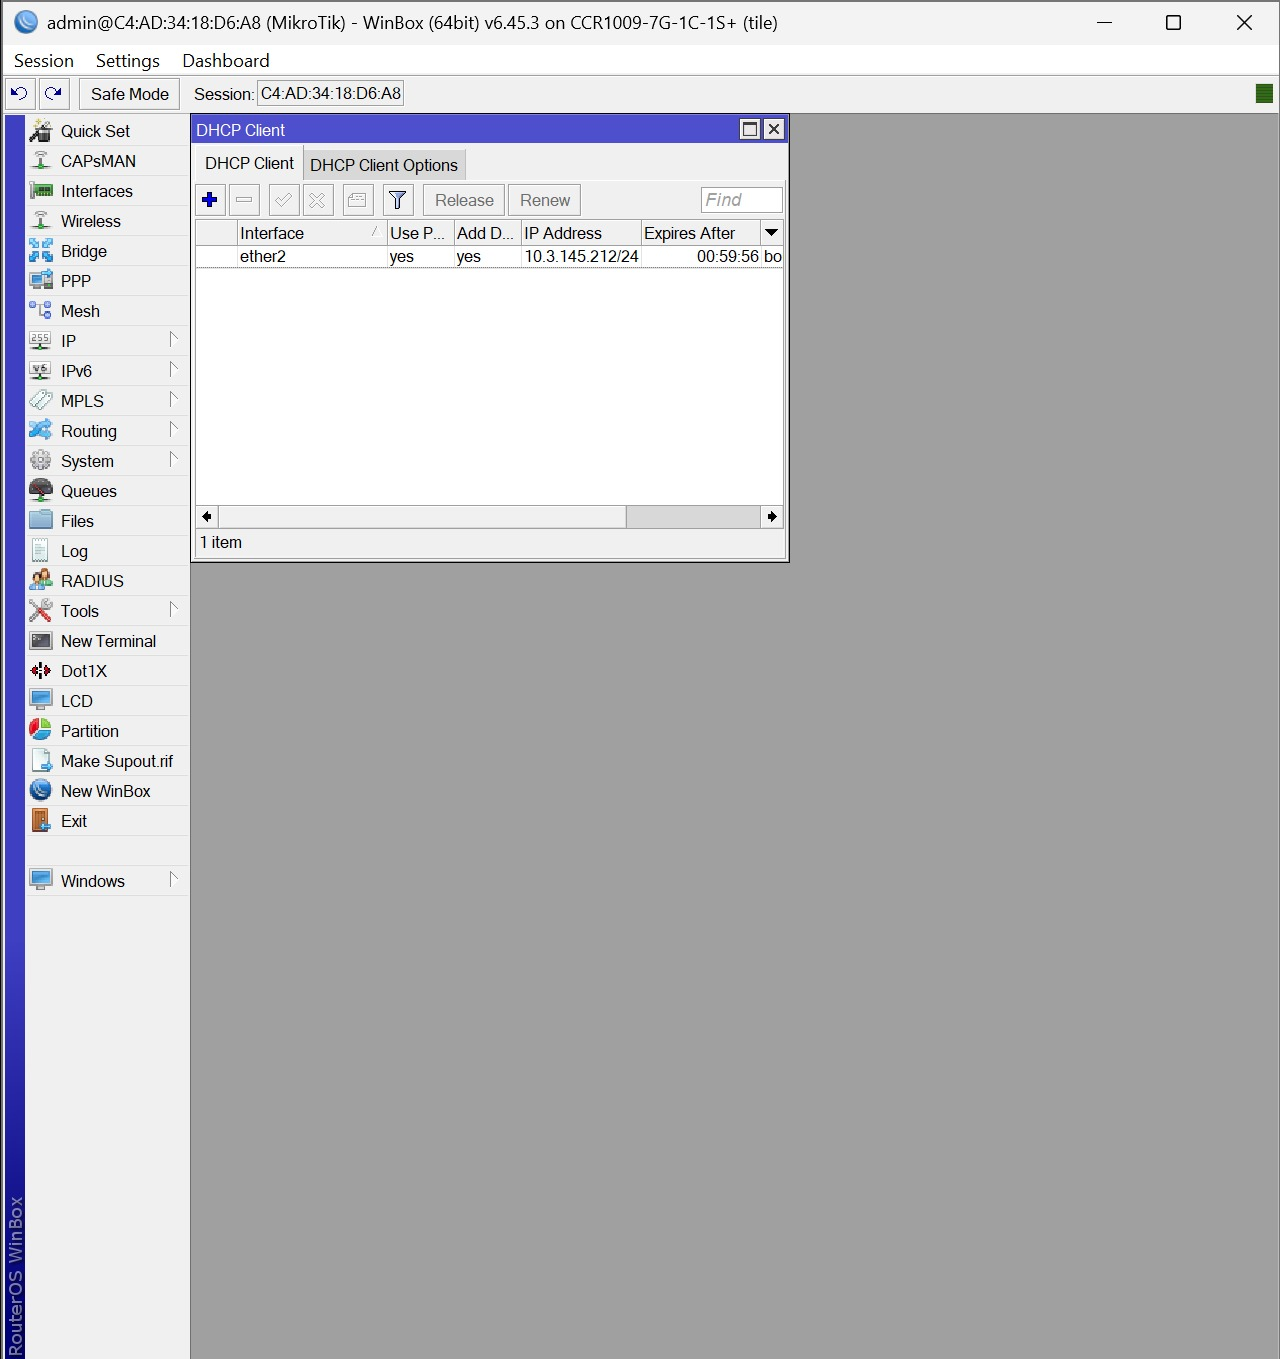
\includegraphics[width=0.5\linewidth]{gambar5.jpeg}
        \caption{Mengkonfigurasikan DHCP server pada mikrotik}
        \label{fig:DHCP-server-mikrotik}
    \end{figure}
    \item Mengaktifkan Proxy ARP
    \begin{figure}[H]
        \centering
        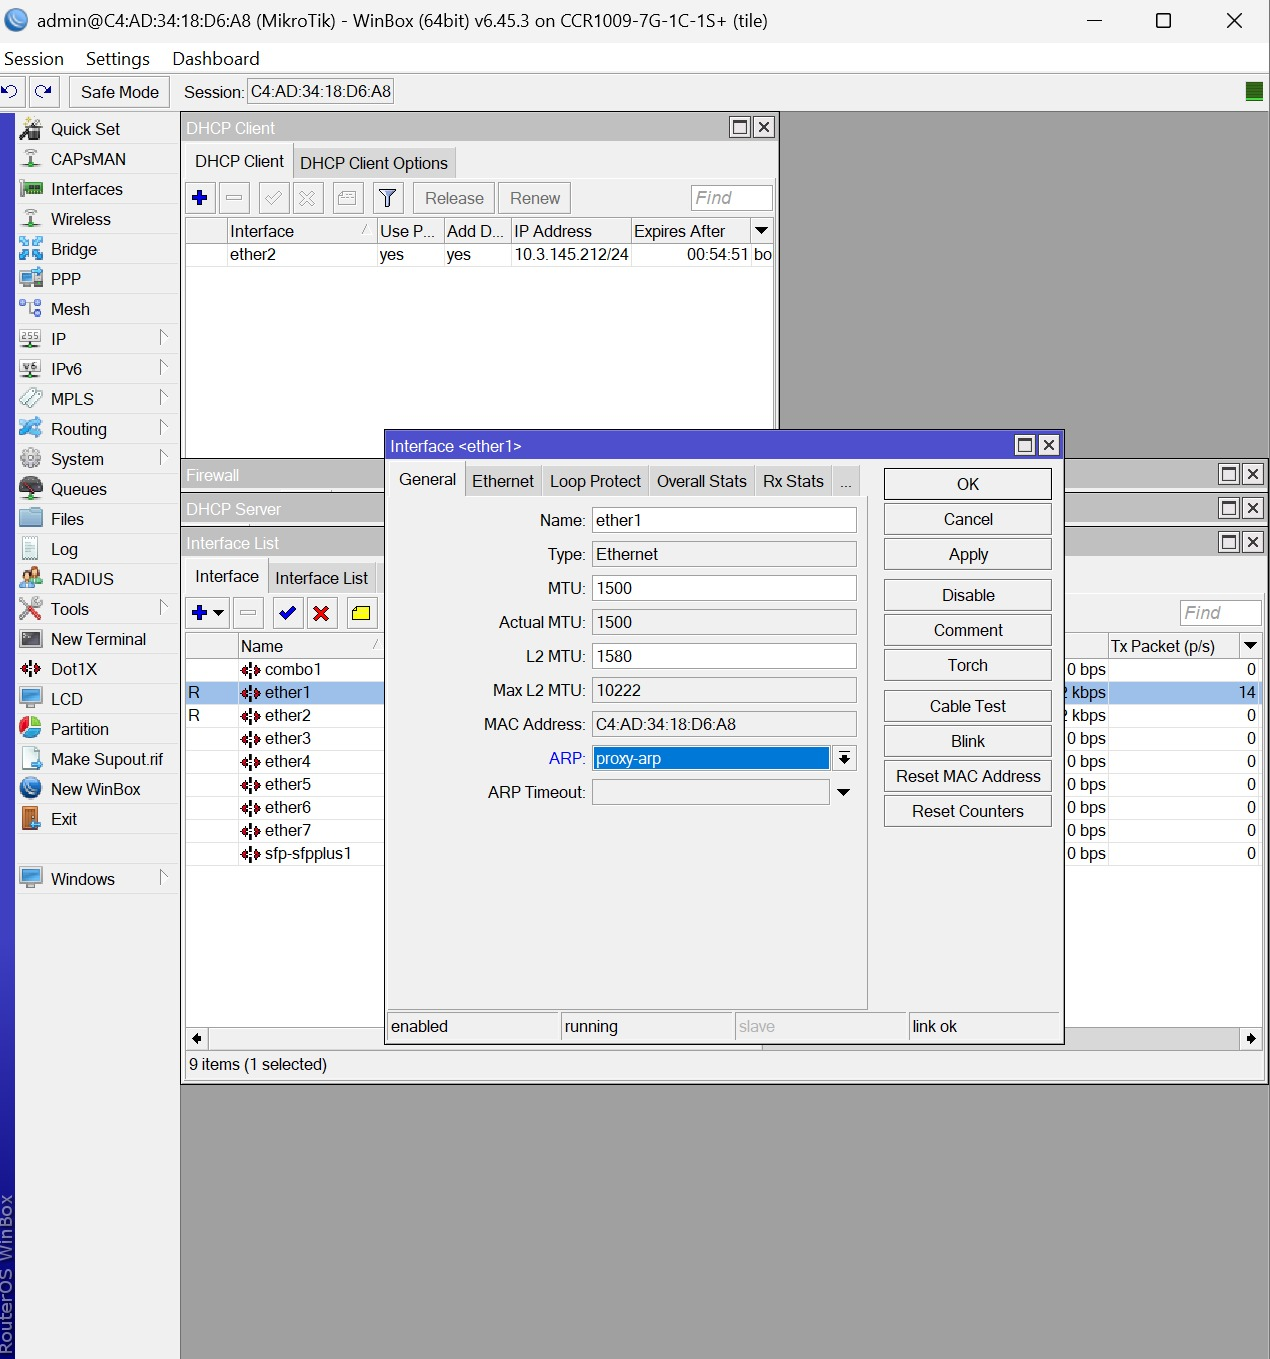
\includegraphics[width=0.5\linewidth]{gambar6.jpeg}
        \caption{Mengaktifkan Proxy ARP}
        \label{fig:Proxy-ARP}
    \end{figure}
    \item Konfigurasi PPTP server
    \begin{figure}[H]
        \centering
        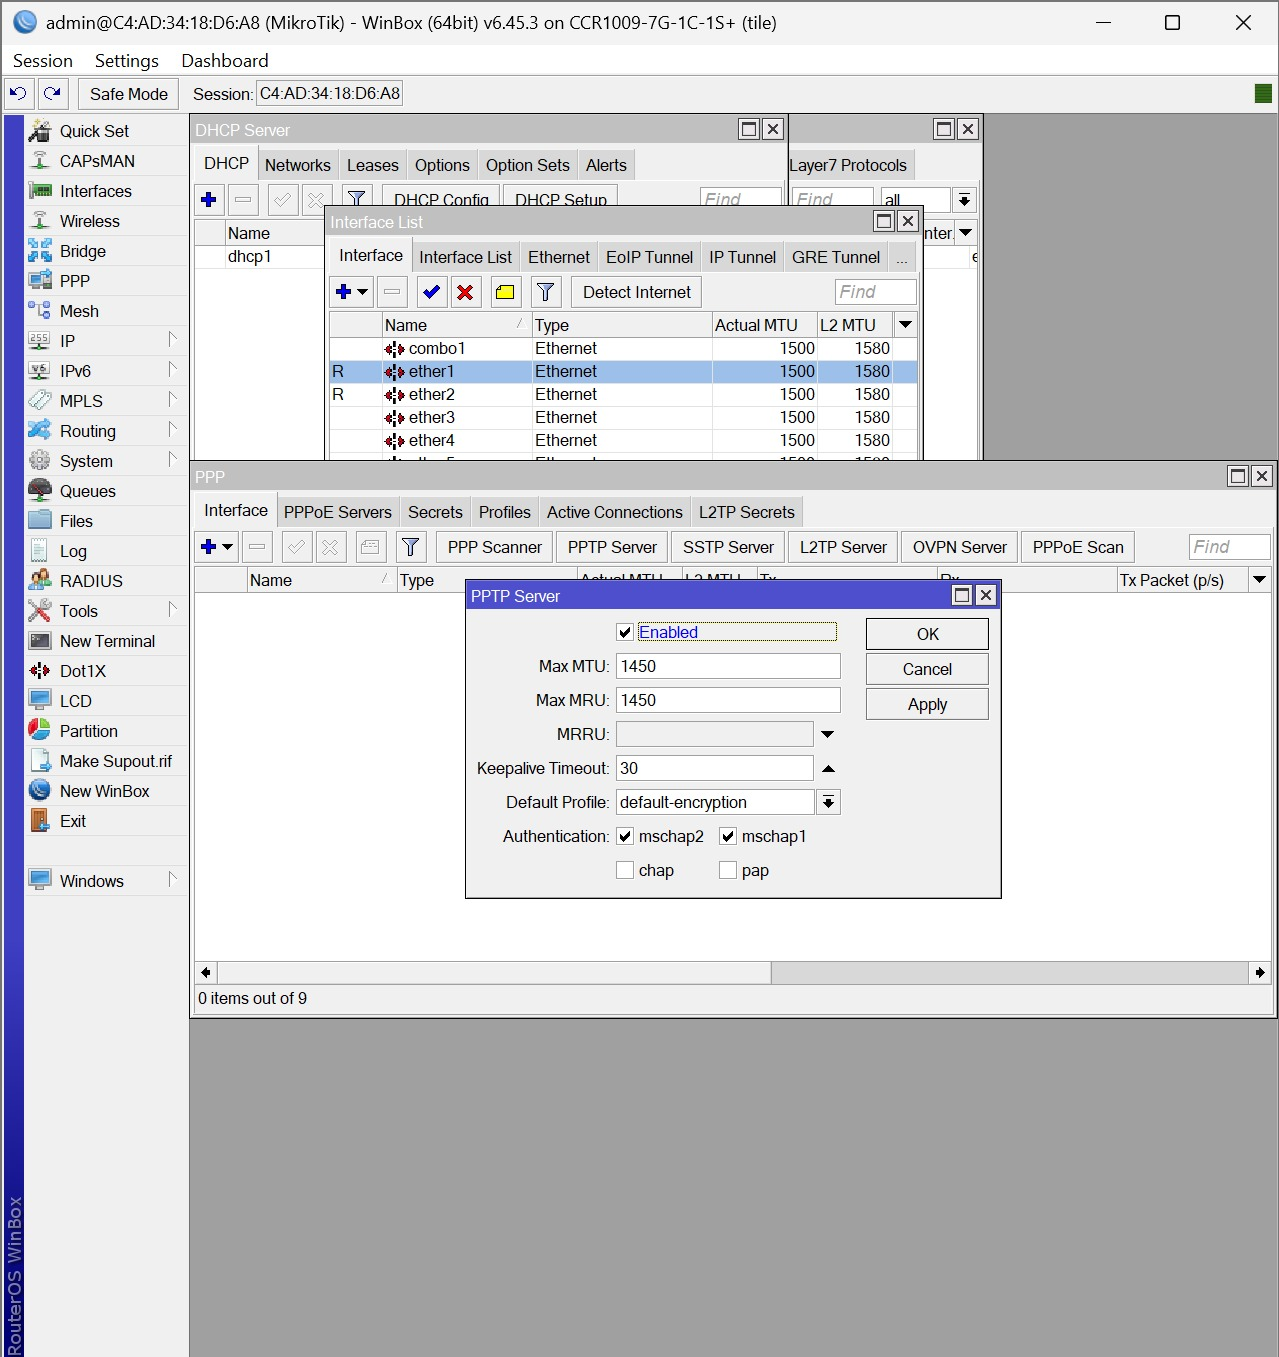
\includegraphics[width=0.5\linewidth]{gambar7.jpeg}
        \caption{Mengkonfigurasi PPTP server pada mikrotik}
        \label{fig:PPTP-server-mikrotik}
    \end{figure}
    \item Membuat User dan password kredensial
    \begin{figure}[H]
        \centering
        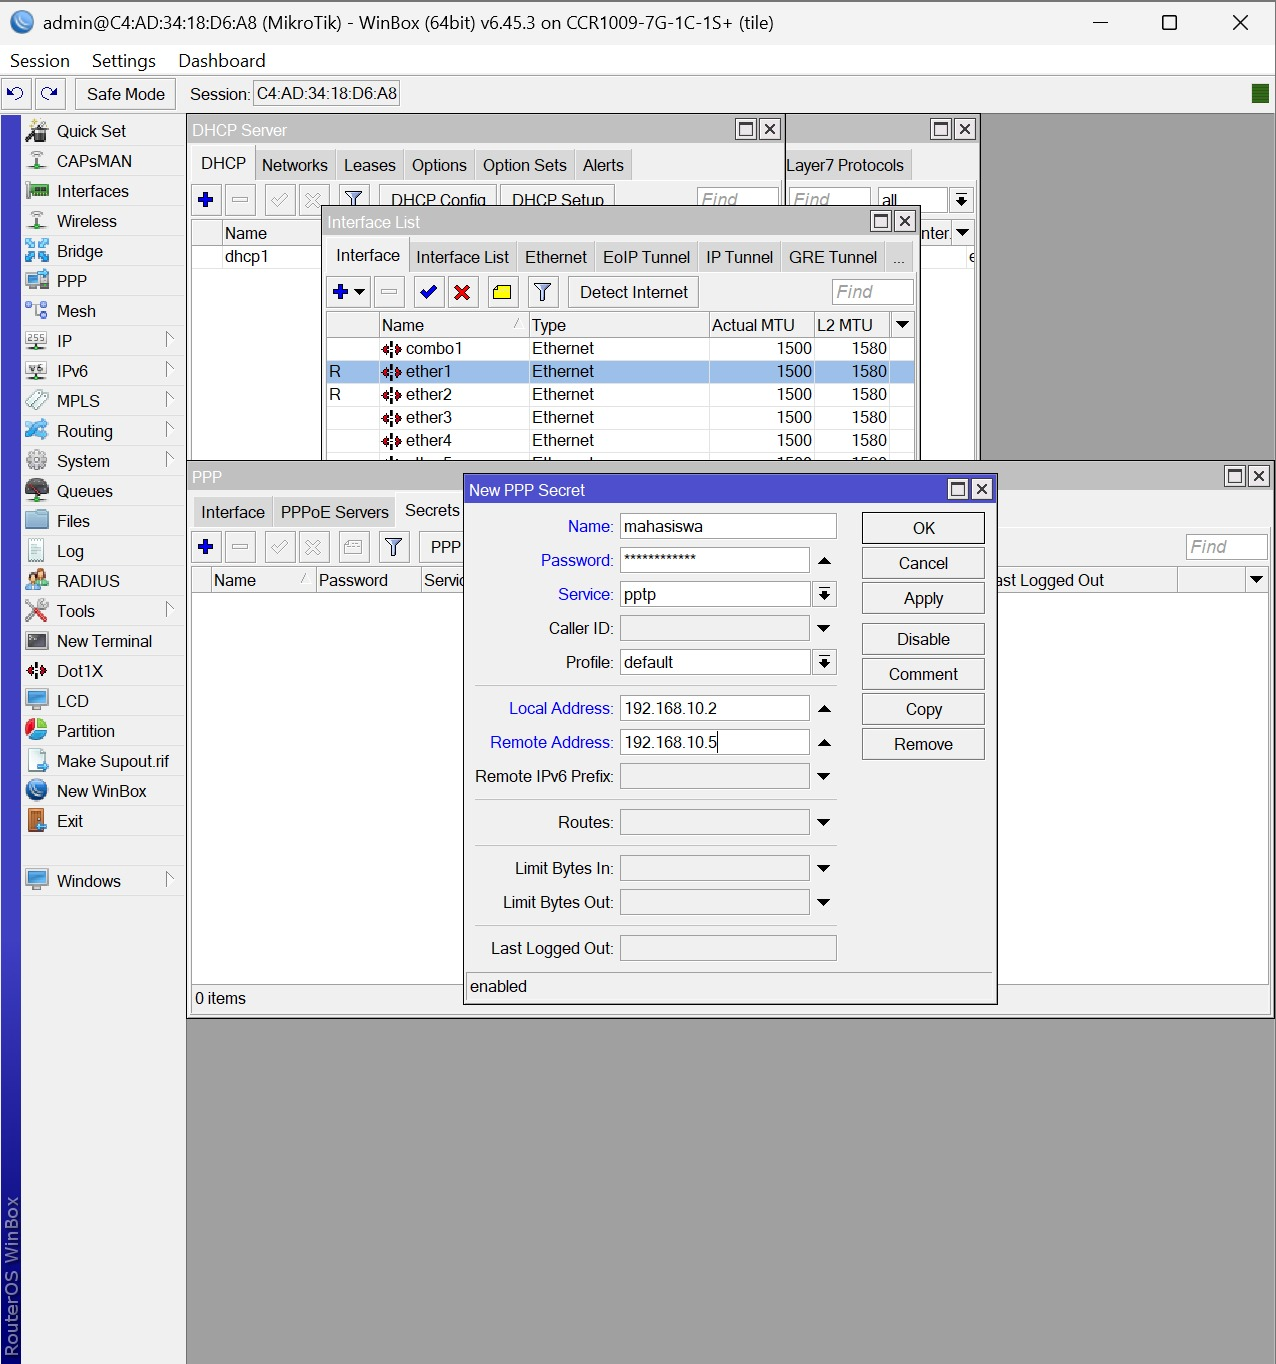
\includegraphics[width=0.5\linewidth]{gambar8.jpeg}
        \caption{Membuat User dan password pada mikrotik}
        \label{fig:User-password-mikrotik}
    \end{figure}
    \item Konfigurasi PPTP client pada laptop
    \begin{figure}[H]
        \centering
        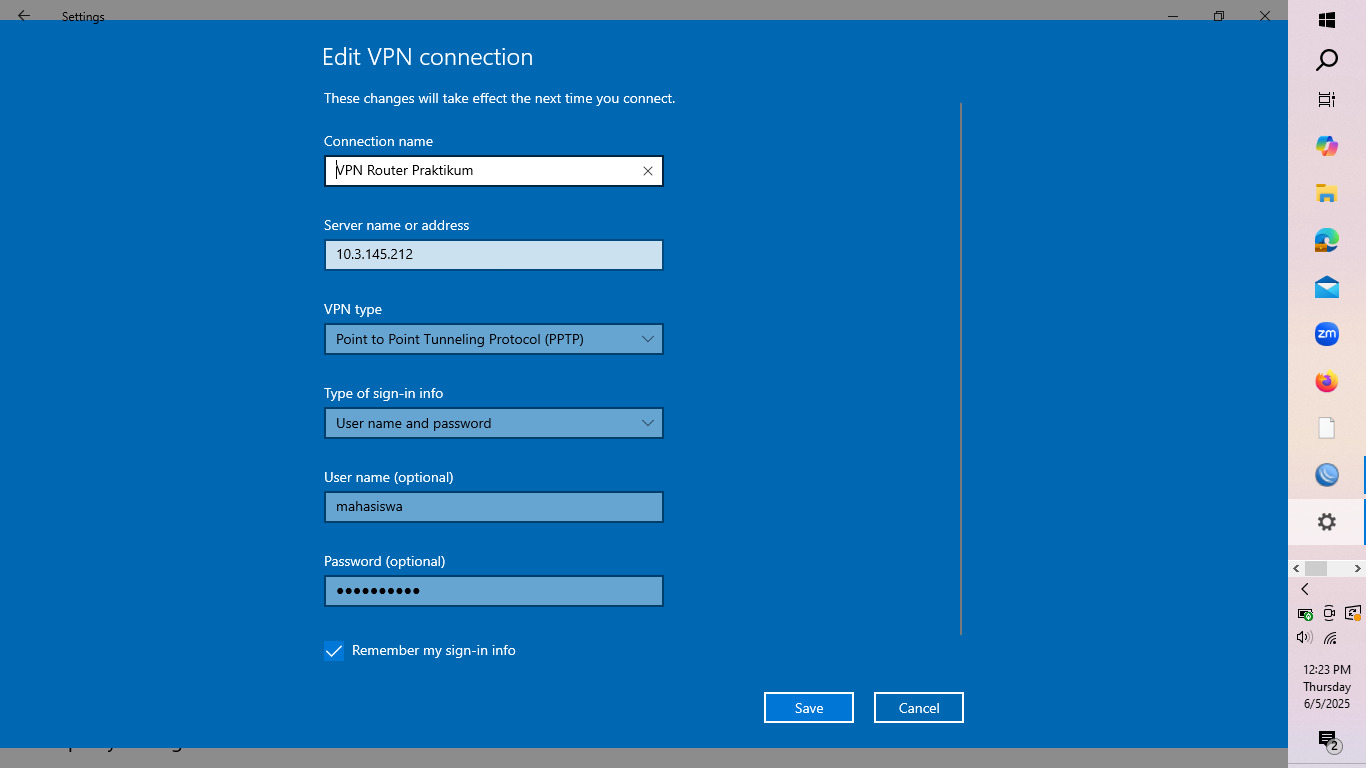
\includegraphics[width=0.5\linewidth]{gambar9.jpeg}
        \caption{Mengkonfigurasi PPTP client pada laptop}
        \label{fig:PPTP-client-laptop}
    \end{figure}
    \item Melakukan verifikasi koneksi 
    \begin{figure}[H]
        \centering
        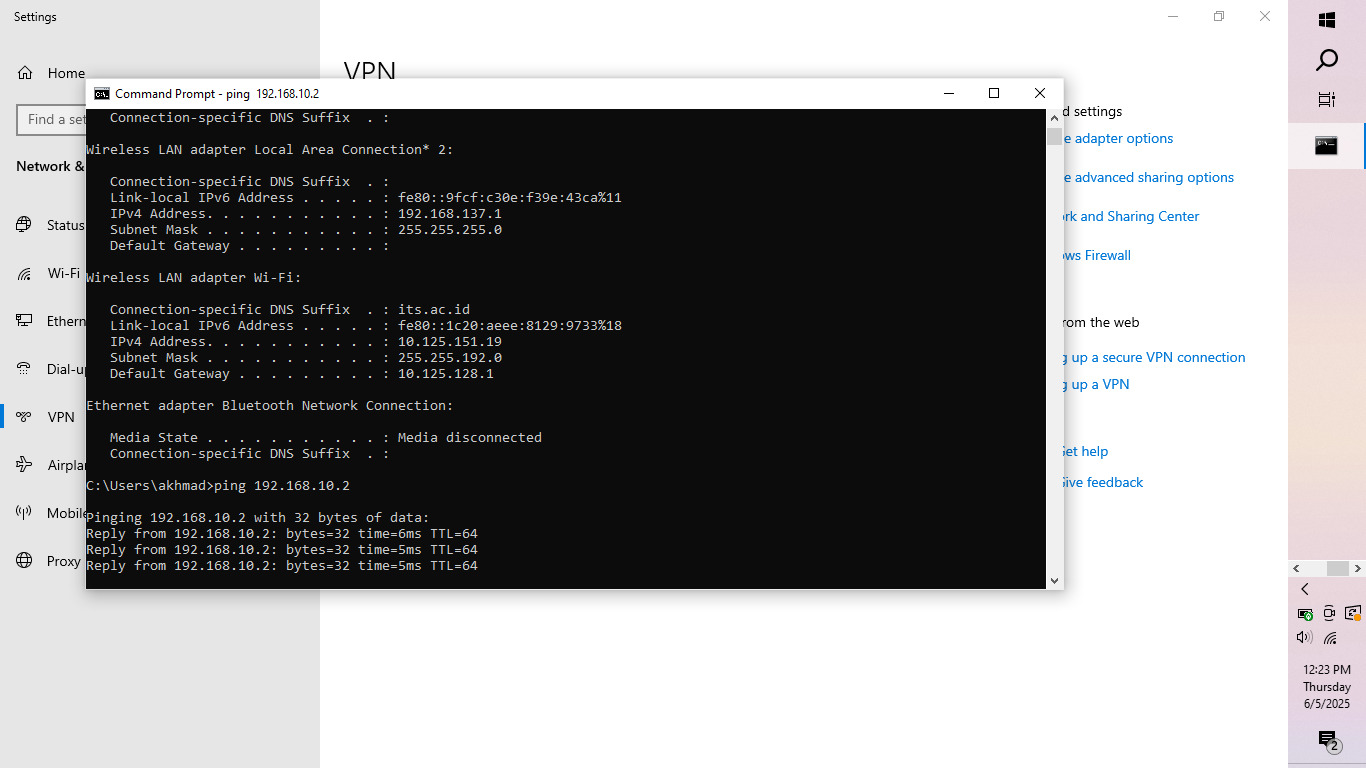
\includegraphics[width=0.5\linewidth]{gambar10.jpeg}
        \caption{Verifikasi koneksi PPTP client pada laptop}
        \label{fig:Verifikasi-koneksi-laptop}
    \end{figure}

    \begin{figure}[H]
        \centering
        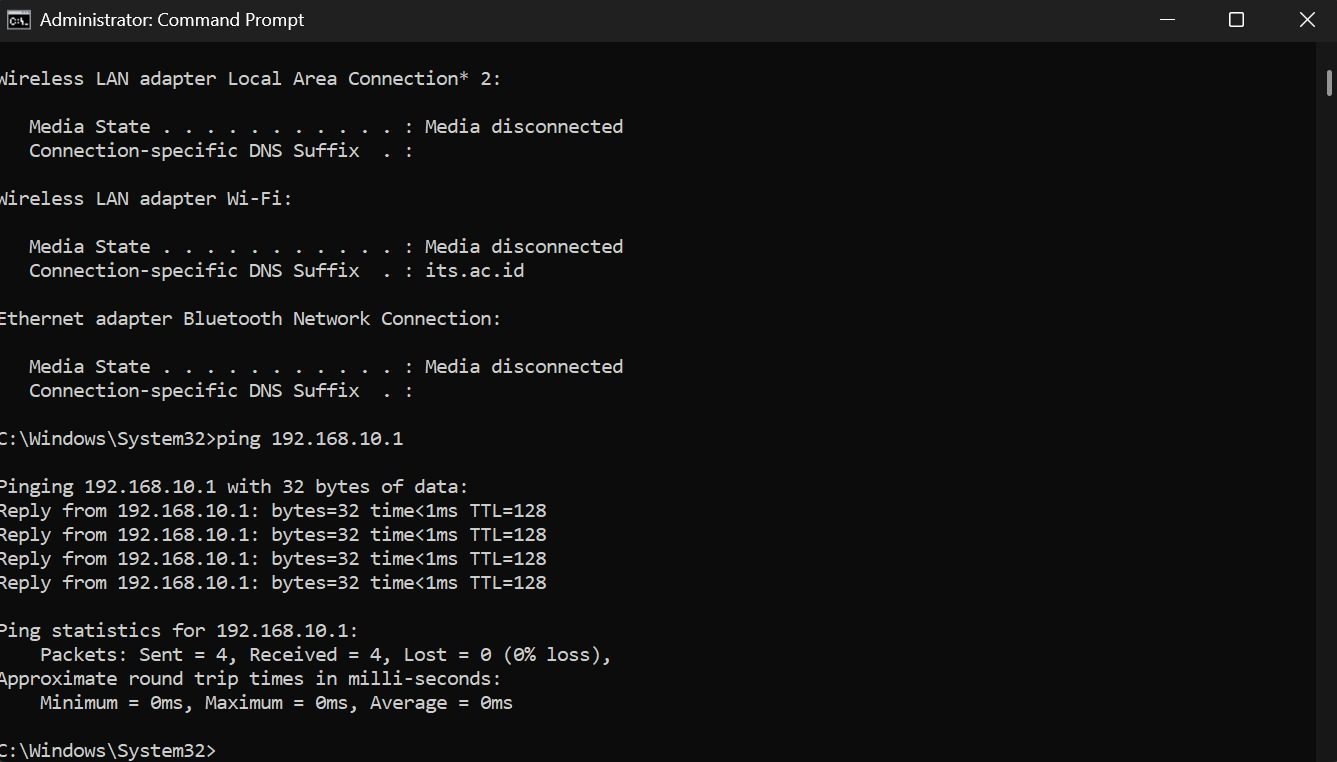
\includegraphics[width=0.5\linewidth]{gambar10b.jpeg}
        \caption{Verifikasi koneksi PPTP client pada laptop}
        \label{fig:Verifikasi-koneksi-laptop}
    \end{figure}


    \item Membuat aturan simple queue untuk membatasi bandwidth
    \begin{figure}[H]
        \centering
        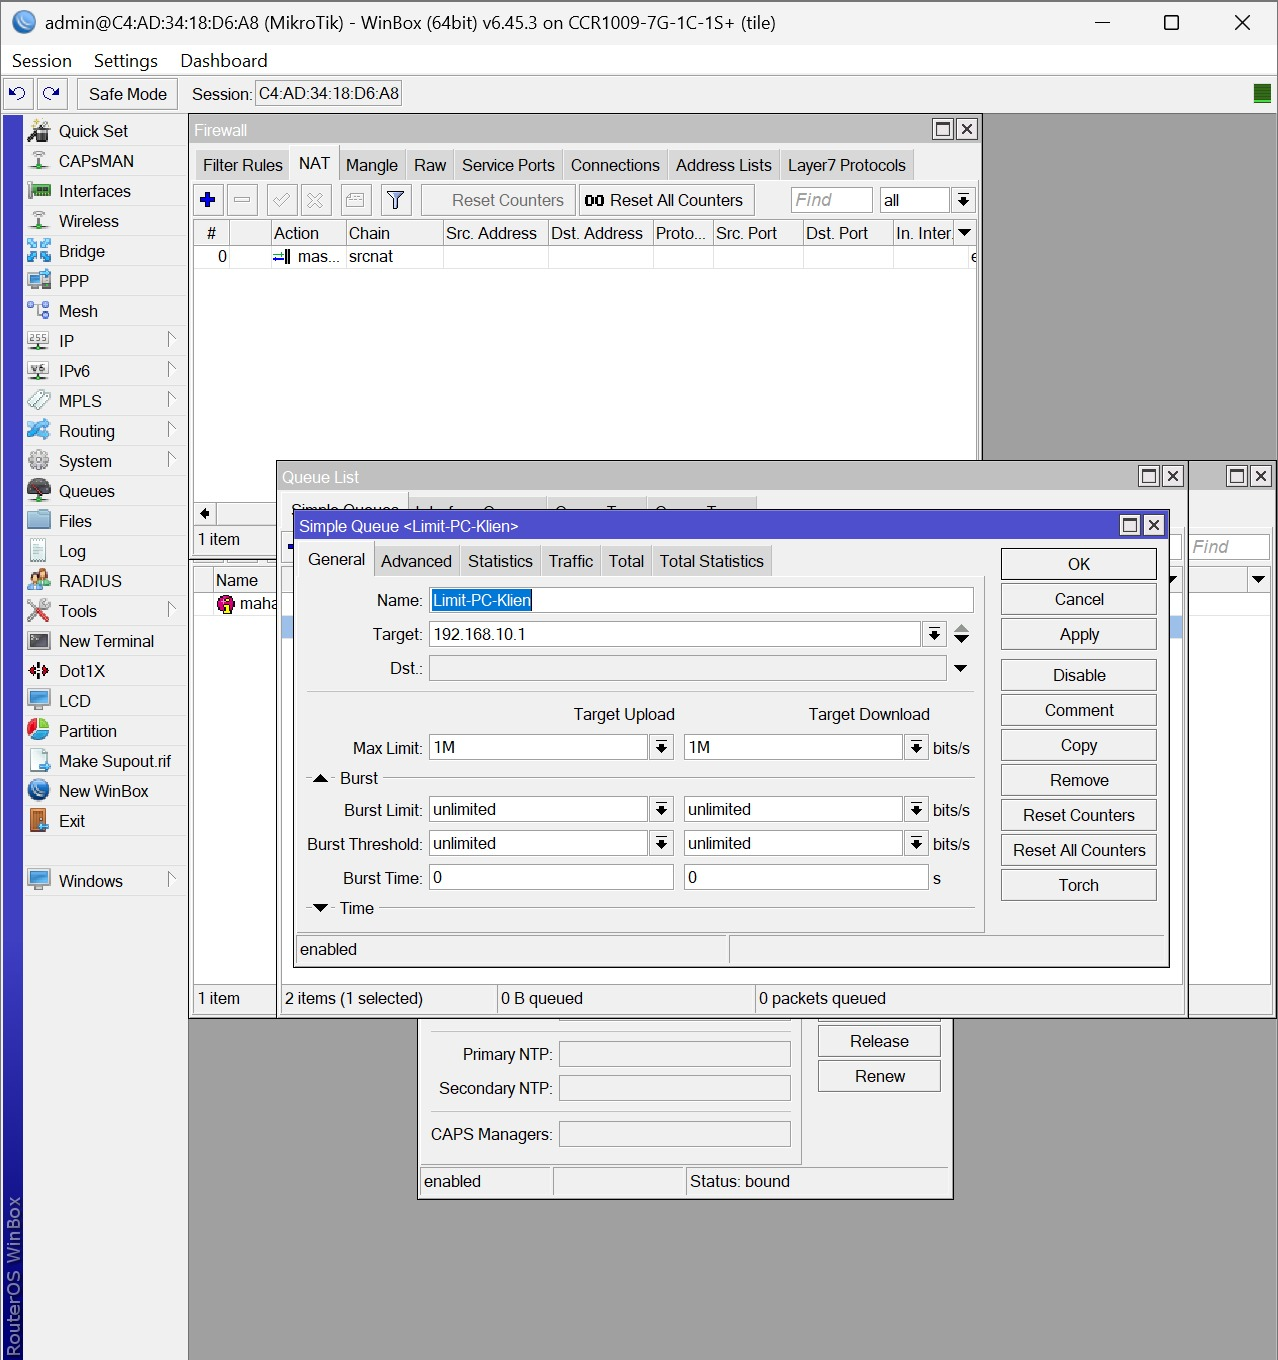
\includegraphics[width=0.5\linewidth]{gambar11.jpeg}
        \caption{Membuat aturan simple queue pada mikrotik}
        \label{fig:Simple-queue-mikrotik}
    \end{figure}
    \item Memantau Penggunaan trafic
    \begin{figure}[H]
        \centering
        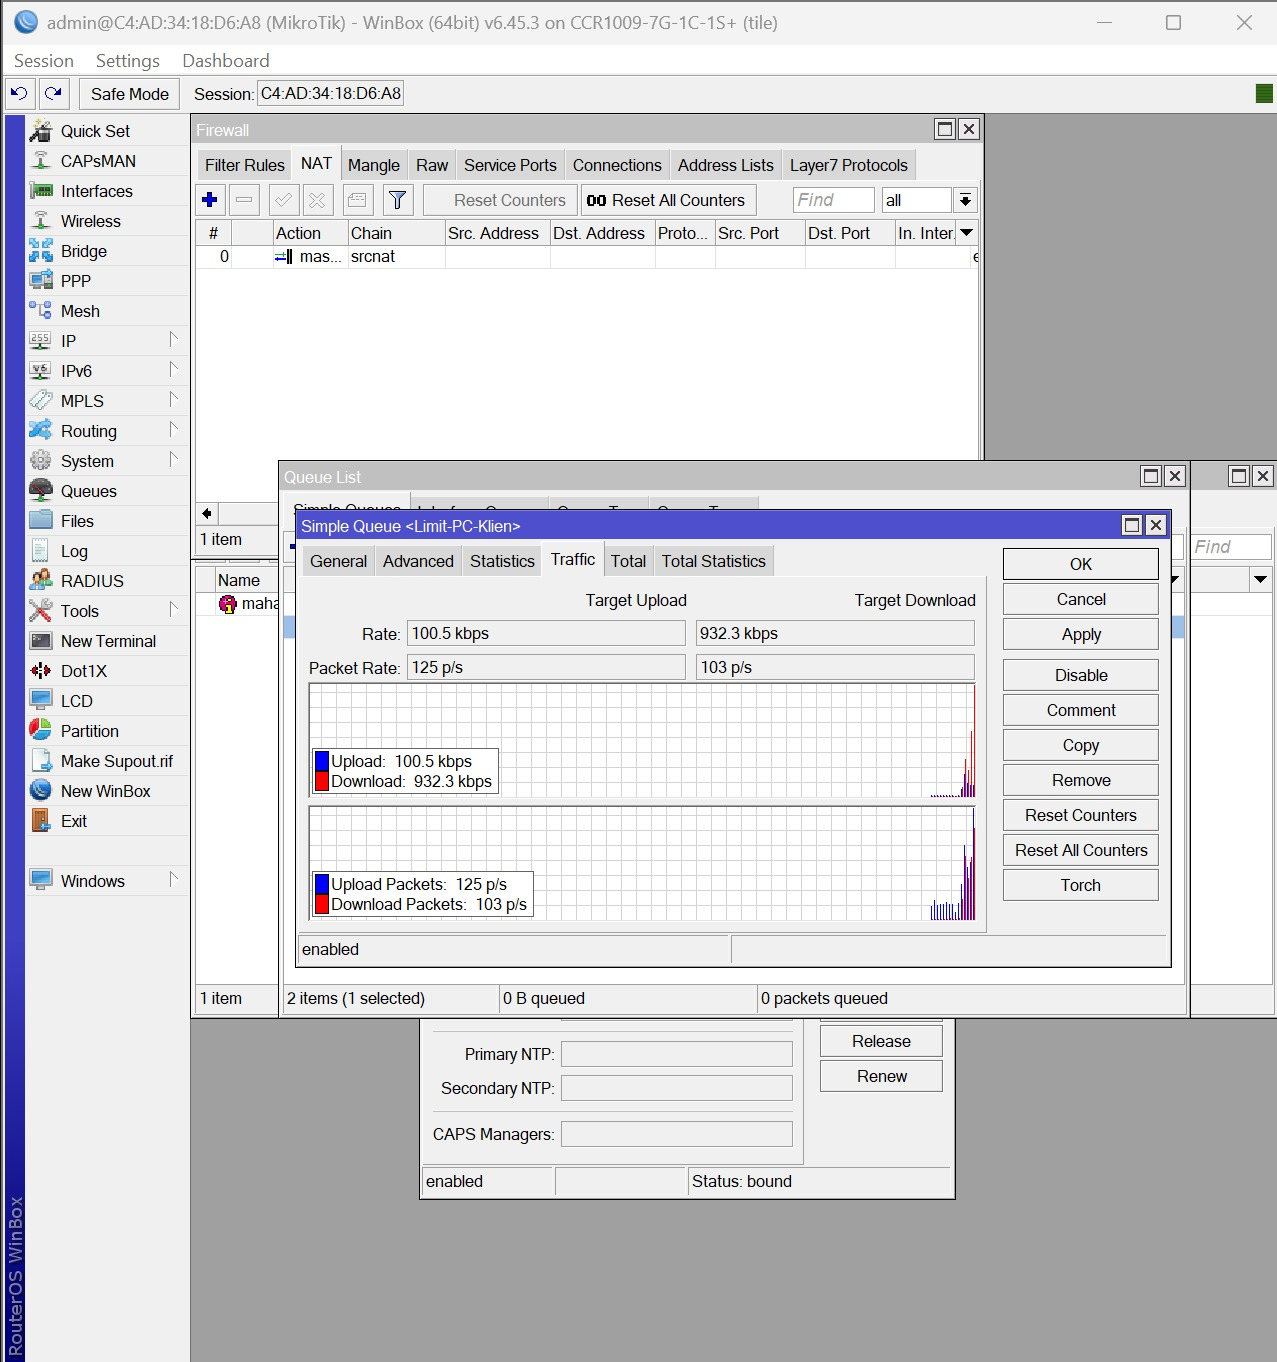
\includegraphics[width=0.5\linewidth]{gambar12.jpeg}
        \caption{Memantau penggunaan trafik pada mikrotik}
        \label{fig:Monitoring-trafik-mikrotik}
    \end{figure}

    \item Pengujian koneksi internet dengan queue
    \begin{figure}[H]
        \centering
        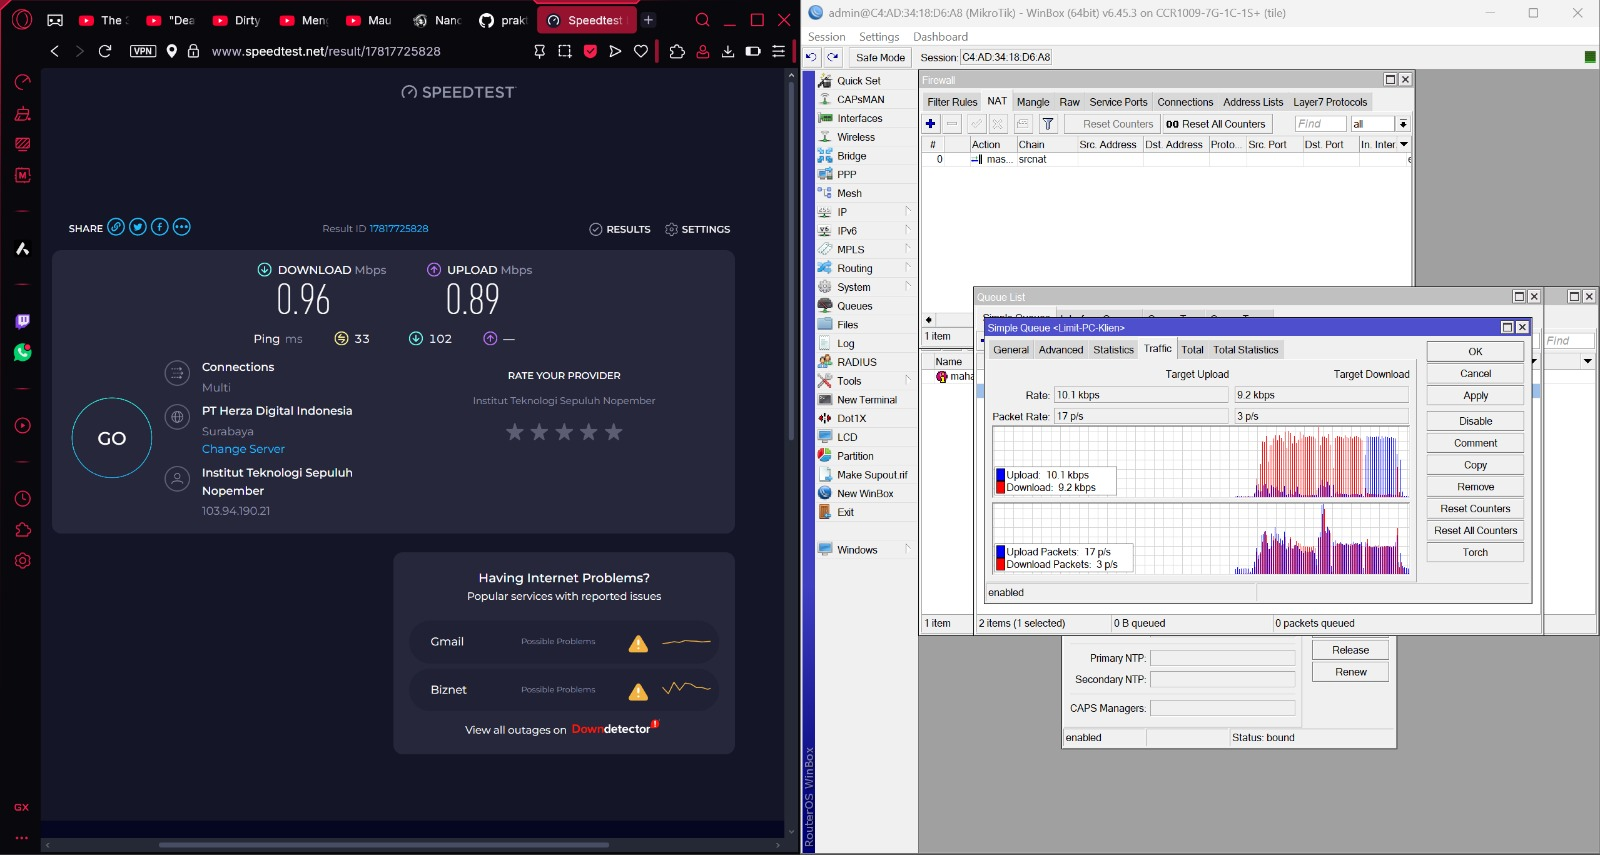
\includegraphics[width=0.5\linewidth]{gambar13.jpeg}
        \caption{Pengujian koneksi internet dengan queue pada mikrotik dengan limitasi bandwidth}
        \label{fig:Pengujian-koneksi-internet-mikrotik}
    \end{figure}

    \begin{figure}[H]
        \centering
        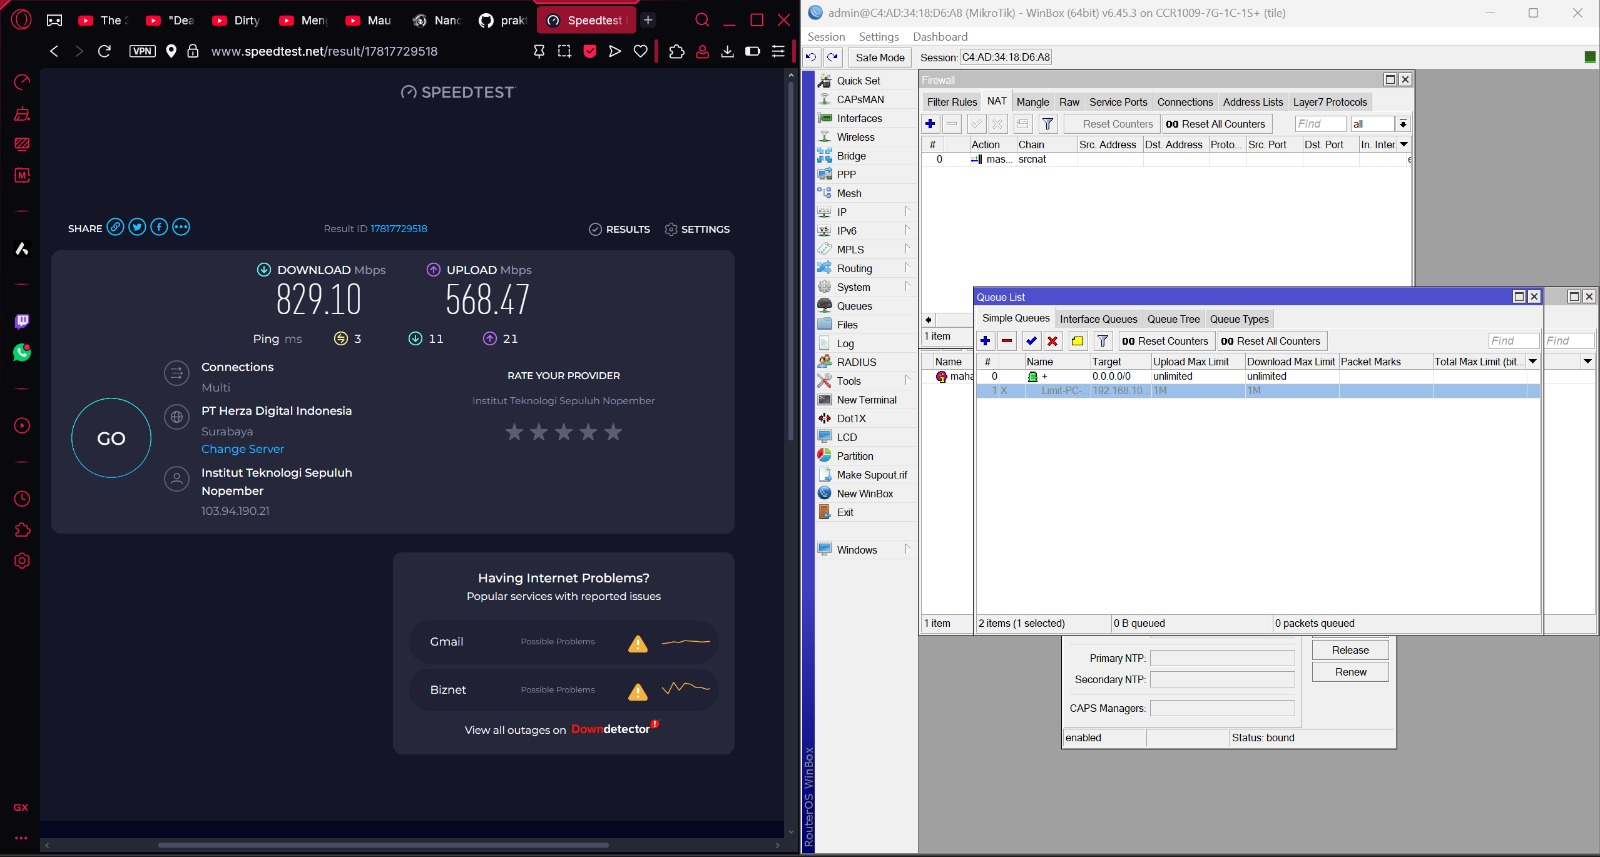
\includegraphics[width=0.5\linewidth]{gambar14.jpeg}
        \caption{Pengujian koneksi internet dengan queue pada mikrotik dengan tidak limitasi bandwidth}
        \label{fig:Pengujian-koneksi-internet-mikrotik-2}
    \end{figure}

\end{enumerate}


\section{Analisis Hasil Percobaan}


Pada percobaan ini, konfigurasi Virtual Private Network (VPN) menggunakan protokol Point-to-Point Tunneling Protocol (PPTP) berhasil dilakukan 
antara laptop dan router Mikrotik. Langkah-langkah seperti mengaktifkan PPTP server, membuat user dan password, serta mengatur PPTP client pada 
laptop menunjukkan hasil yang positif, ditandai dengan keberhasilan verifikasi koneksi antara perangkat klien dan server VPN. Koneksi VPN ini 
memungkinkan klien untuk mengakses jaringan lokal secara aman melalui jalur terenkripsi, meskipun berada pada jaringan yang berbeda. Hal ini 
berguna untuk kebutuhan akses jaringan internal dari jarak jauh, dengan jaminan keamanan data melalui tunneling.

Selain itu, konfigurasi Quality of Service (QoS) melalui fitur \textit{simple queue} juga berhasil diimplementasikan. Dengan menetapkan batas 
bandwidth tertentu pada user yang terhubung, Mikrotik mampu mengelola dan mengalokasikan sumber daya jaringan secara efisien. Hasil pengujian 
menunjukkan bahwa bandwidth klien dapat dikendalikan sesuai parameter yang telah ditentukan, sehingga penggunaan jaringan menjadi lebih adil dan 
terkontrol. Monitoring trafik juga memberikan visualisasi penggunaan bandwidth secara real-time, yang sangat membantu dalam proses evaluasi 
performa jaringan dan identifikasi bottleneck. Implementasi kombinasi antara VPN dan QoS ini menunjukkan bagaimana Mikrotik dapat digunakan 
untuk membangun jaringan yang aman dan efisien, baik untuk kebutuhan skala kecil maupun menengah.

\section{Hasil Tugas Modul}

    \begin{figure}[H]
        \centering
        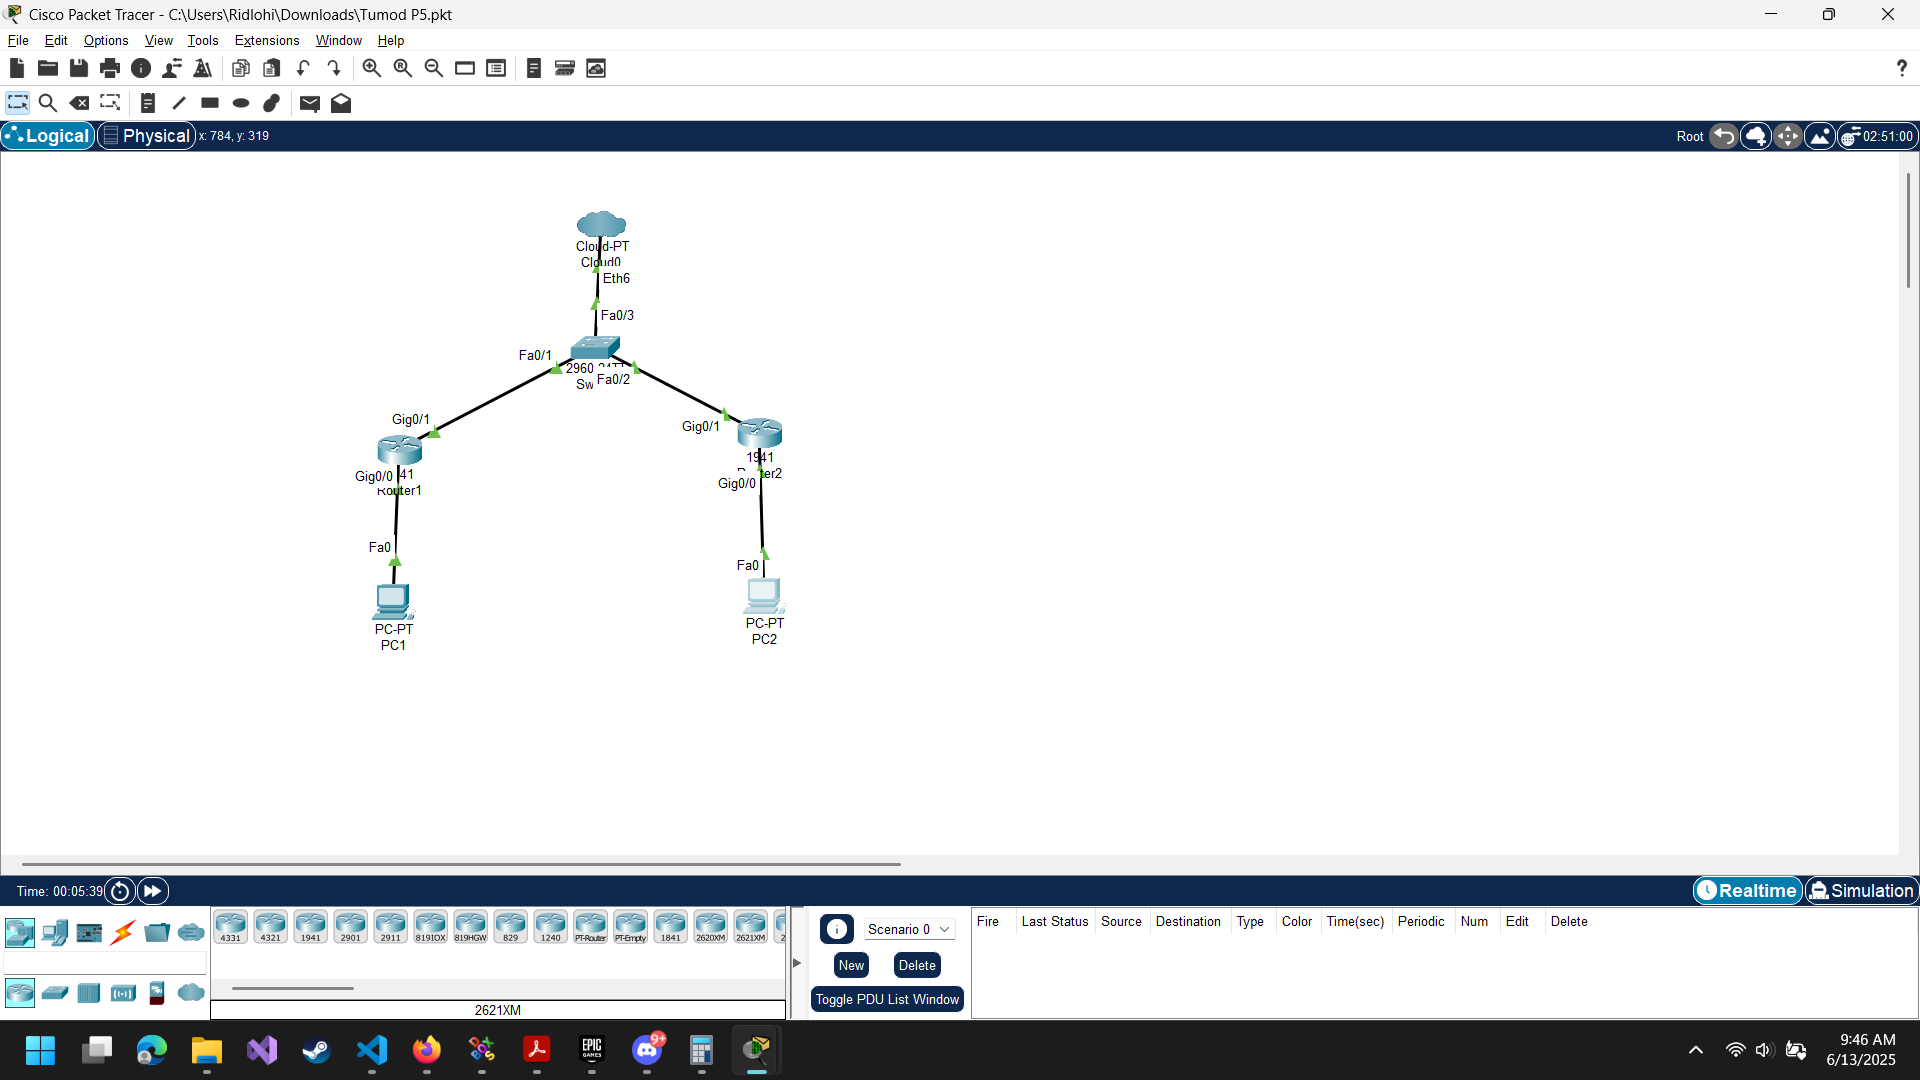
\includegraphics[width=0.5\linewidth]{tumod1.png}
        \caption{Topologi jaringan}
        \label{fig:Topologi-jaringan}
    \end{figure}

    \begin{figure}[H]
        \centering
        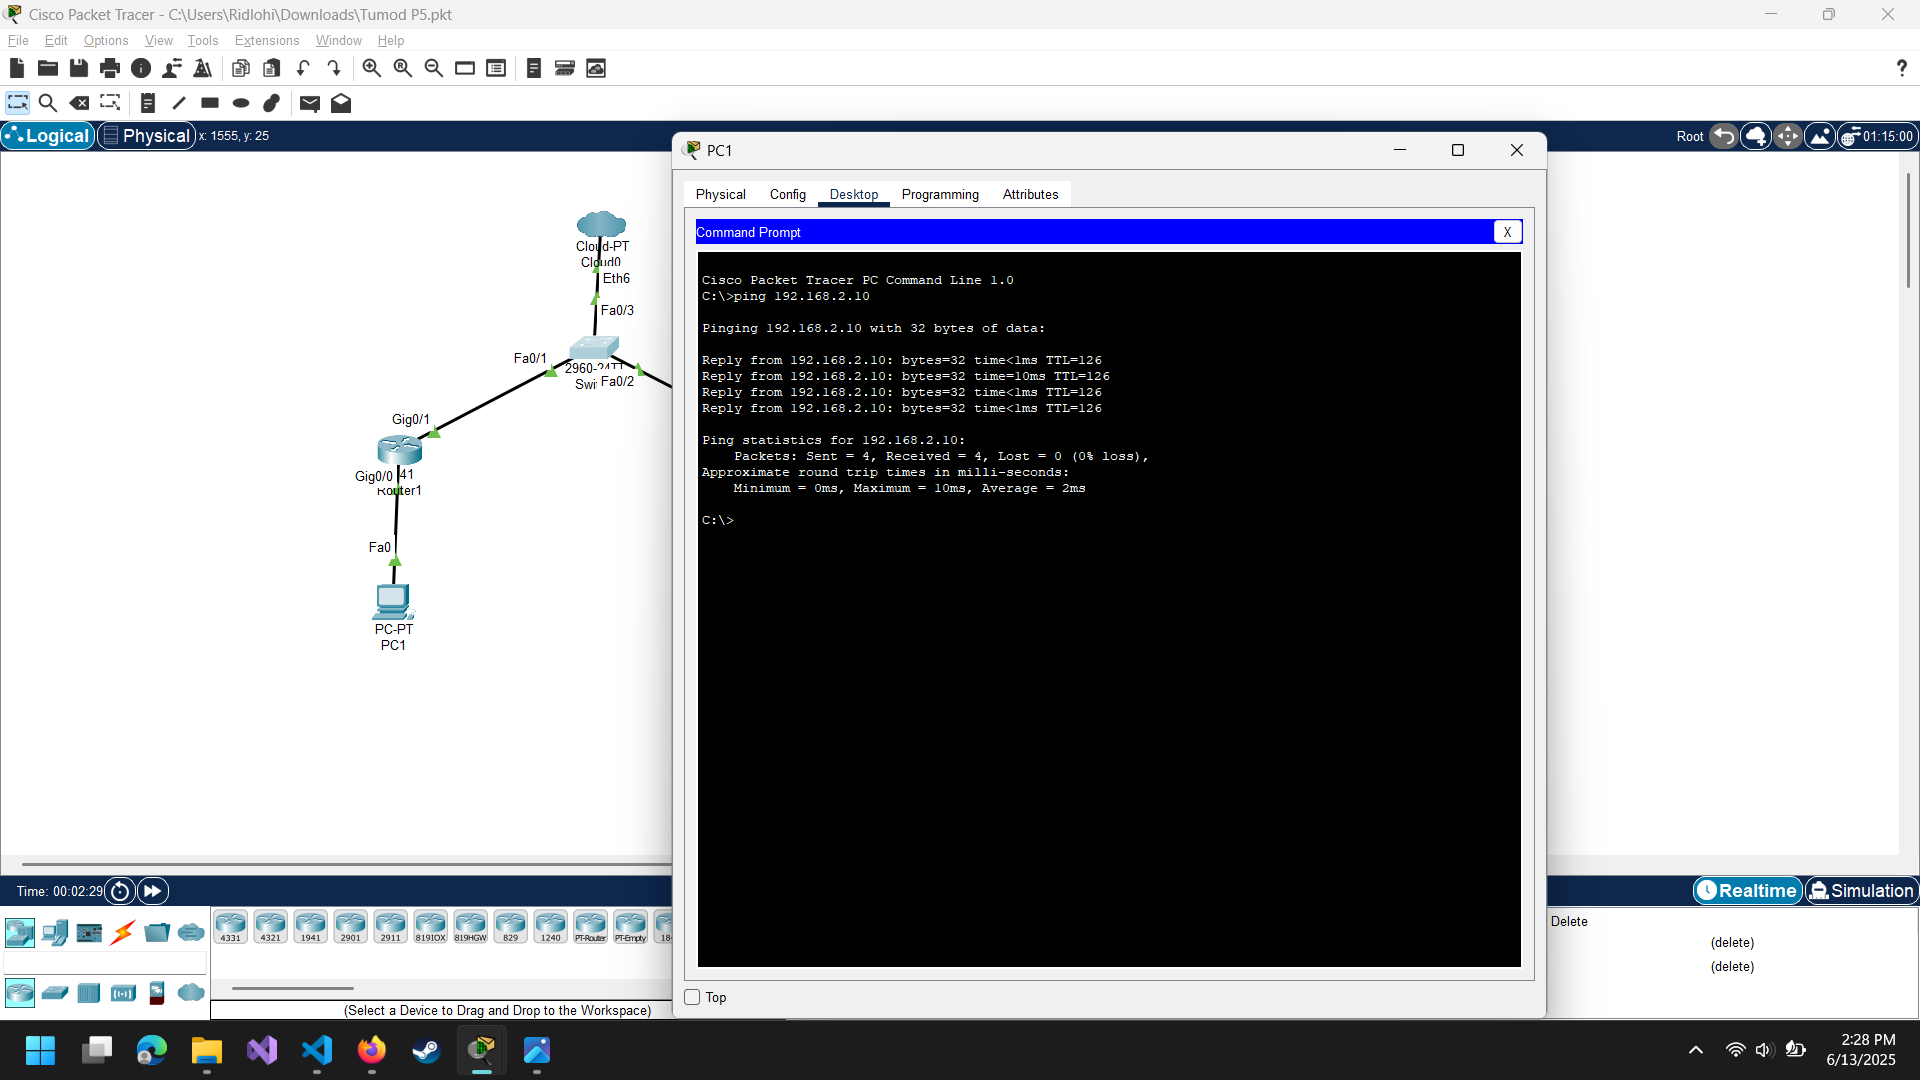
\includegraphics[width=0.5\linewidth]{tumod2.png}
        \caption{Uji ping}
        \label{fig:Pengujian-koneksi}
    \end{figure}

    \begin{figure}[H]
        \centering
        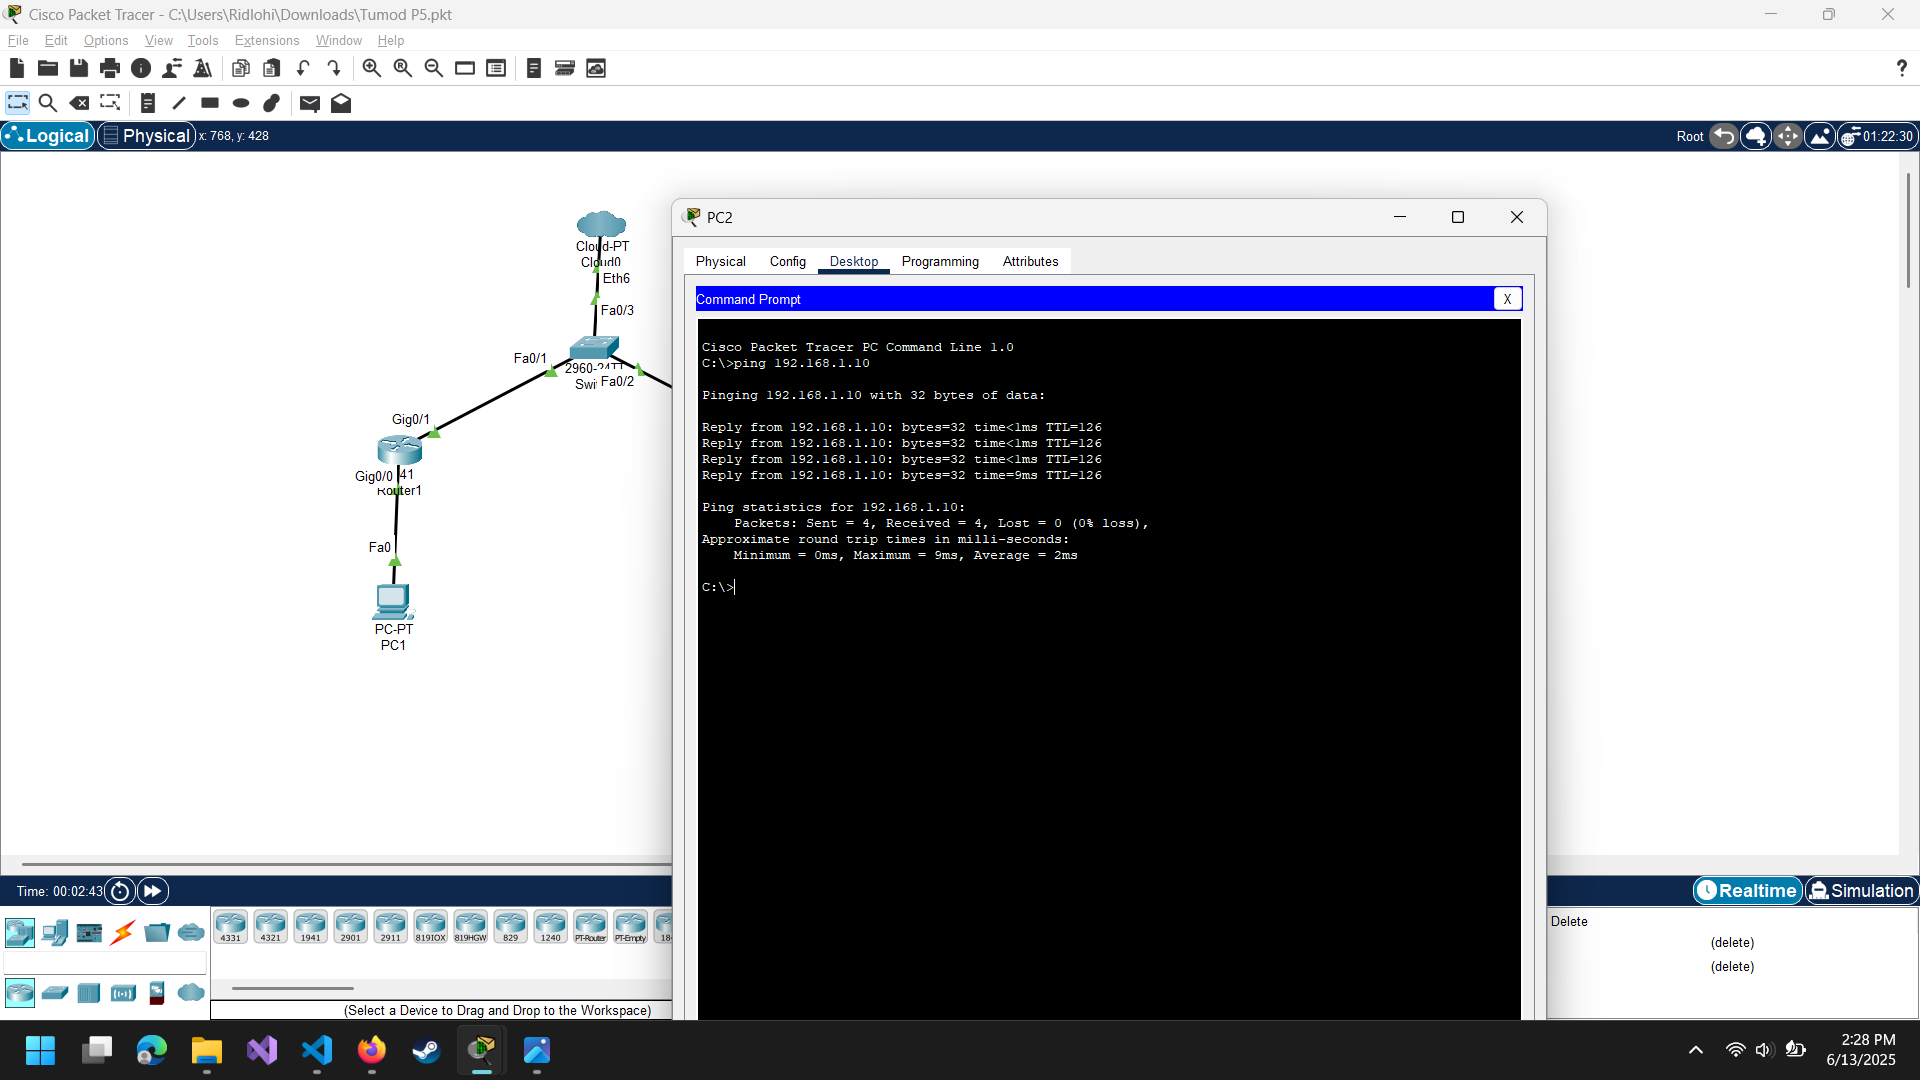
\includegraphics[width=0.5\linewidth]{tumod3.png}
        \caption{Uji ping}
        \label{fig:Pengujian-koneksi}
    \end{figure}

Dalam simulasi ini, PPTP (\textbf{Point-to-Point Tunneling Protocol}) menciptakan terowongan
virtual antara Router 1 dan Router 2 di atas jaringan publik (Internet).
Fungsinya adalah memungkinkan komunikasi aman dan privat antara PC1 dan PC2,
seolah-olah mereka berada dalam satu jaringan lokal yang sama.
PPTP membungkus paket data dari satu sisi jaringan
dan mengirimkannya melalui terowongan tersebut ke sisi lain,
meskipun data secara fisik melewati jaringan yang tidak aman.

\section{Kesimpulan}
Seteleah melakukan praktikum ini, dapat disimpulkan bahwa VPN (Virtual Private Network) dengan protokol PPTP (Point-to-Point Tunneling Protocol) 
berhasil diimplementasikan dan VPN  berguna untuk  mengamankan koneksi jaringan dan mampu mengakses jaringan lokal dari jarak jauh.
Selain itu, konfigurasi Quality of Service (QoS) menggunakan fitur \textit{simple queue} pada Mikrotik berhasil dilakukan, yang memungkinkan
pengaturan bandwidth untuk setiap user. Hal ini membantu dalam mengelola trafik jaringan secara efisien, memastikan bahwa sumber daya jaringan digunakan secara optimal. 

\section{Lampiran}
\subsection{Dokumentasi saat praktikum}

    \begin{figure}[H]
        \centering
        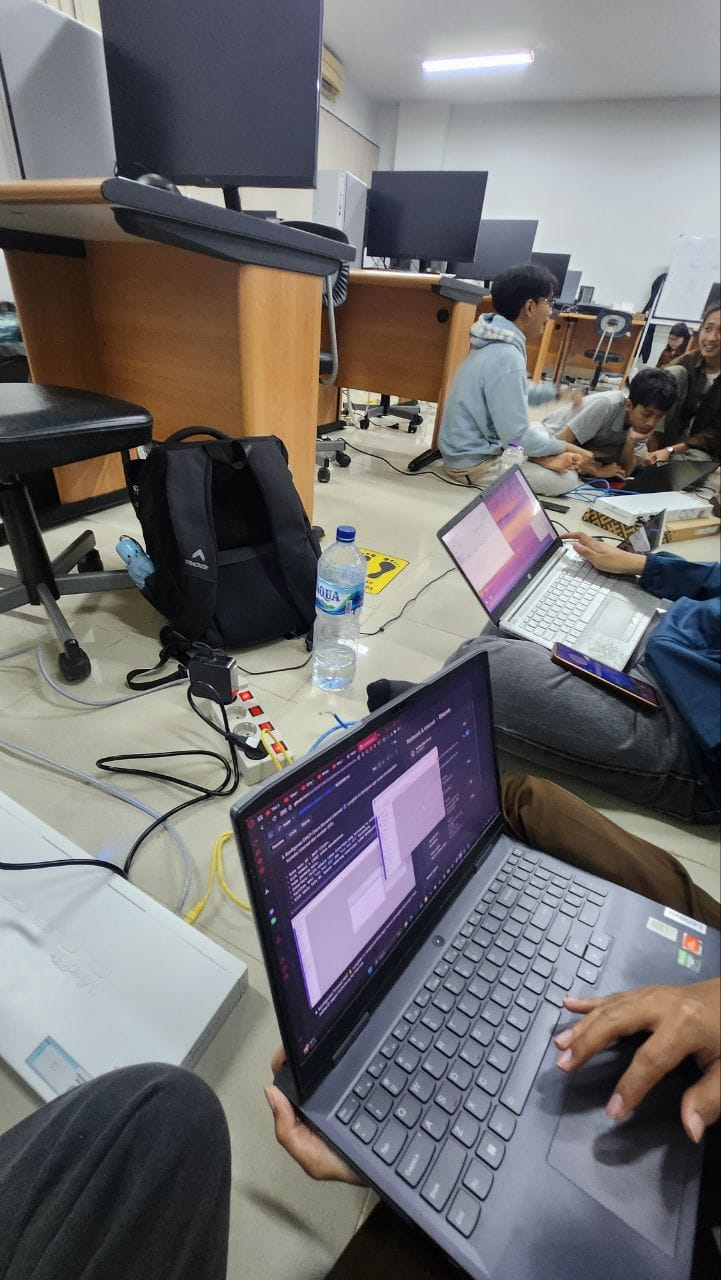
\includegraphics[width=0.5\linewidth]{lampiran.jpeg}
        \caption{Lampiran}
        \label{fig:Lampiran}
    \end{figure}

